% !TEX root = ../main.tex

\chapter{绪论}
\section{研究背景和意义}
自然界中许多生物具有群体行为\cite{couzin2005effective},例如狮群的协作捕食、大雁的成行飞行、鱼类的聚集洄游等。
这些生物个体并没有人类那样的智慧与能力,每个个体与其他个体的信息交流能力也并不出色,
但正是这样一个个简单弱小的个体,却能形成强大的群体组织,完成复杂而多样的群体任务。

\begin{figure}[!htp]
    \centering
    \begin{minipage}{0.48\textwidth}
      \centering
      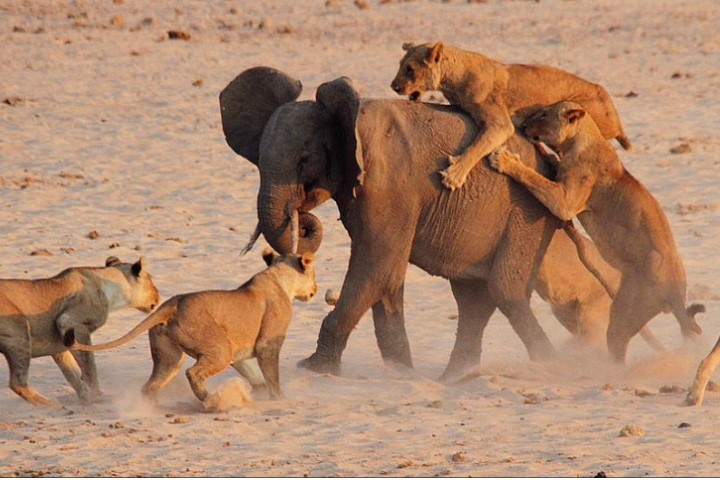
\includegraphics[height=4.5cm]{lion.jpg}
      \caption{狮群的协作捕食}
      \label{fig:lion}
    \end{minipage}\hfill
    \begin{minipage}{0.48\textwidth}
      \centering
      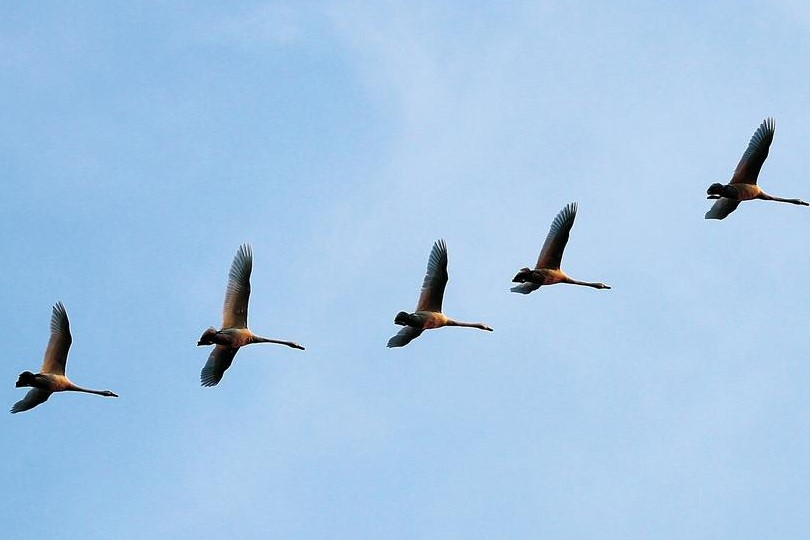
\includegraphics[height=4.5cm]{dayan.jpeg}
      \caption{大雁的成行飞行}
      \label{fig:dayan}
    \end{minipage}
  \end{figure}

在人类生产生活中,也常有协作完成任务的场景,例如车辆编队\cite{ren2008distributed}、分布式传感\cite{lesser2003distributed}、机器人协作\cite{ismail2018survey}等。
人们越来越认识到,相比单个强大而复杂的个体,多个简单个体的合作往往能以更小的代价完成任务。
因此,多智能体系统(\textbf{Multi-Agent Systems, MASs})这一理论模型从自然科学、工程学中抽象出来,引起了越来越多研究者的兴趣。
构成系统的每个智能体具有自己的运行逻辑,从环境中或从其他智能体处获得信息,并作出相应的变化。
智能体之间的信息交互通常受限,且具有独特的交互方式。
智能体各自的运行逻辑,也称作动力学,往往也是复杂而多样。
为了在诸多限制中控制多智能体系统合作完成任务,多智能体协同控制这一子领域应运而生。

多智能体协同控制主要的研究目标有:1.设计分布式的控制协议,仅利用每个智能体从其他智能体处获得的少量信息,进行协同行动;
2.针对各种各类复杂的限制条件,例如故障、攻击、通讯间隔、通讯延迟等,进一步研究并提升控制协议的抗扰性、鲁棒性;
3.探寻协作合作与隐私保护之间的平衡。
多智能体协同控制的研究结合了网络科学、控制科学、计算机科学、数学等多个领域,
需要用到图论、矩阵理论、优化理论等多方面的知识,具有很强的交叉性。

多刚体系统是一类特殊的多智能体系统,系统中的每个智能体为刚体模型,其运行逻辑服从刚体动力学。
刚体是一种理想模型,在外力作用下不会发生形变,刚体的运动包含平动与转动。
飞机、船舶、航天器等人类生产生活中的大量装置均可抽象为刚体模型,因此对多刚体系统的研究,可以应用到这些装置的编队与协作实践中。

近年来无人机集群吸引了人们大量目光,其中用到的不仅仅有无人机的位置协同控制,
还包含了姿态控制,以保证在狭窄严酷的环境中仍能保持编队。
由于小型航天器的发展与发射成本的降低,航天器的编队协作具有广泛的应用与发展前景\cite{long2021distributed}\cite{jin2023synchronization},
一组小型的卫星能以更小的总成本完成一颗大型卫星所不能完成的任务,
例如天基红外干涉阵列、分布式深空观测等,这些应用要求各个航天器姿态一致(或特定朝向)。
从以上两个例子可以看出,刚体模型相比质点模型多出的三个转动自由度增加了刚体的灵活性,
也赋予了多刚体系统完成更加复杂任务的能力,因此多刚体系统姿态控制是多刚体系统实现功能的重要一环。
\begin{figure}[!htp]
    \centering
    \begin{minipage}{0.48\textwidth}
      \centering
      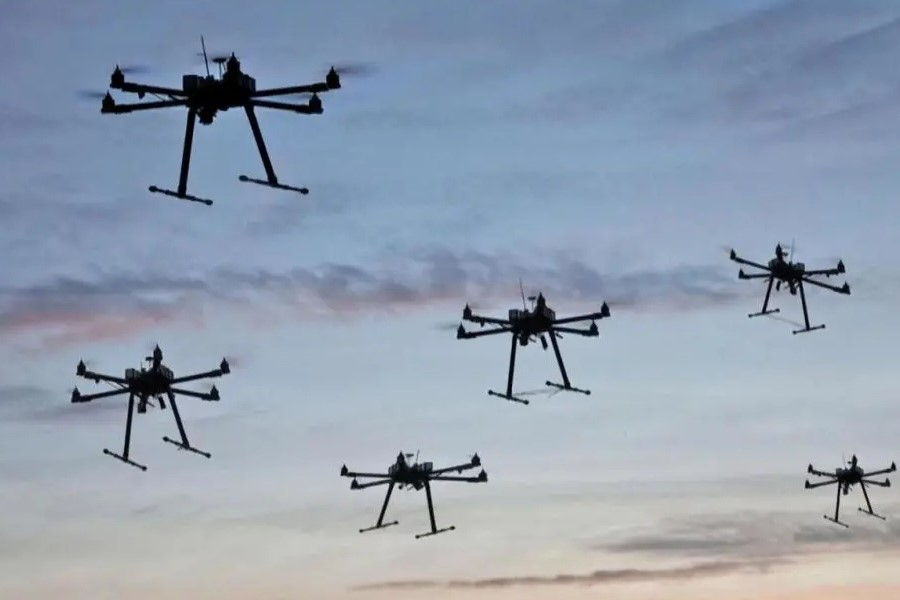
\includegraphics[height=4.5cm]{uav.jpg}
      \caption{无人机集群}
      \label{fig:uav}
    \end{minipage}\hfill
    \begin{minipage}{0.48\textwidth}
      \centering
      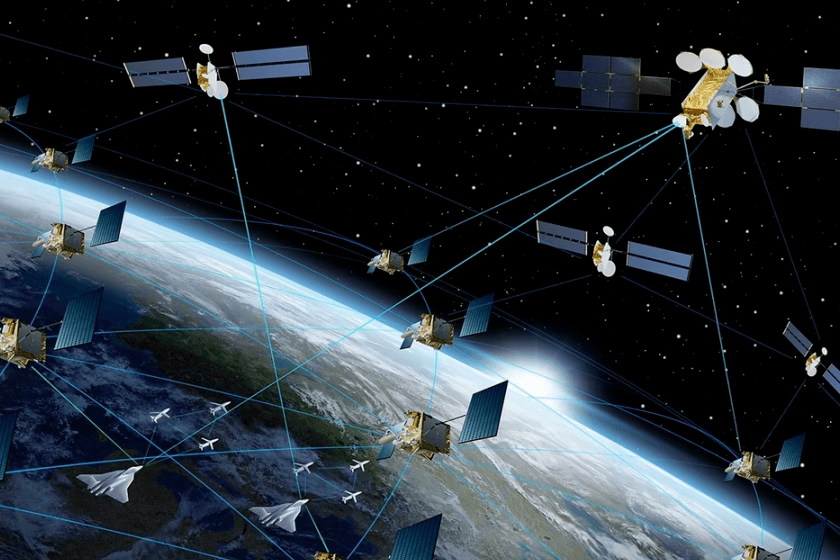
\includegraphics[height=4.5cm]{satellite.png}
      \caption{航天器编队示意图}
      \label{fig:satellite}
    \end{minipage}
  \end{figure}

三个转动自由度的引入,同时也增加了对多刚体系统协同控制研究的挑战性。
姿态(旋转)的变化规律并不是线性的,举一个简单的例子。
先绕$x$轴旋转$\pi/3$再绕$y$轴旋转$\pi/4$得到的姿态,与先绕$y$轴旋转$\pi/4$再绕$x$轴旋转$\pi/3$得到的姿态不相同,
这意味着交换律在姿态问题上是不存在的,因此,我们也不能对姿态求平均值。
这样的数学特性源于旋转空间是一个李群$\text{SO(3)}$\cite{sola2018micro},对加法不封闭,
所以许多处理线性问题的数学方法在姿态系统控制问题上不能使用,需要引入其他的数学工具。
为此,研究者们使用了各种参数来描述旋转,借用微分几何中的定理辅助分析。
相比位置控制,姿态控制是刚体控制研究中更具特色且难度更大的部分,因此本文研究聚焦于多刚体系统姿态协同控制。

总之,多刚体系统姿态协同控制是一个具有广泛应用前景和重要科学意义的问题。
一方面,海、空、天等多层次、多样化的人造装置都具有协作完成任务的需要,多智能体系统理论的一些研究已经广泛应用于各种场景,
而多刚体系统姿态协同控制能为更复杂的任务提供高效的控制策略。
另一方面,针对姿态控制这一非线性控制问题的研究,可以为控制理论非线性问题的处理带来新的理论和方法,
也能为微分几何中的动力学问题提供新的思路。

\section{多刚体姿态一致性的研究现状}

\section{本文研究动机}
\section{本文研究内容和章节安排}
